% !TEX root = UAV_Landing_Pad.tex

\chapter{Sprint Reports}

\section{Sprint Report \#1}

\let\stdsection\section
\renewcommand\section{\newpage\stdsection}

Weeks Sept. 22, 2014 to Oct. 10, 2014:

Teams InSight (Joseph Lillo, Daniel Nix \& Elizabeth Woody) and Eye In The Sky (Colter Assman, Julian Brackins, Charles Parsons \& Alex Wulff) paired to research common design considerations, goals and architecure dependencies.  During this sprint, the following topics were researched: 

	\begin{enumerate}

		\item Development Operating System
 
Both teams required a foundational operating system for the development of our independent software solutions. For familiarity linux was selected as the developing kernel; the distribution was selected as Ubuntu for its integration with robotics documentation and support for Robotics Operating Systems (ROS). Version 14.04 was selected as it was the most current of the long-term support (LTS) editions available. The attempt to run Ubuntu as a virtual machine (VM) posed too many problems to be viable - webcam access was difficult, general performance was greatly reduced, etc. - so dedicated installations were made on laptops and desktops for development.

\item Common API

As Eye In The Sky would be utilizing UGV/UAV technologies and InSight would be utilizing a small deployable Odroid-like computers, a common API would greatly benefit the teams. It was found that keeping with Ubuntu and ROS, nearly all separate software dependencies could be installed to this common platform and reduce the need for redundant research.

\item Computer Vision

Both teams have a need for computer aided recognition of visual queues. To this end, the software package openCV was selected for its integration with ROS based solutions as well as the ability to customize the variations of triggers to be recognized. This software was built into the workspaces used by both team's ROS installations.

\item Verbal \& Auditory Interaction

While not immediately apparent to the needs of Eye In The Sky, verbal interaction was a requirement for the customer experience of InSight. After much deliberation, the package PocketSphynx based on CMU Sphynx was accepted for the light size, functionality, C++ integration and extended customization options that this solution provides over alternatives like SpeechLion or Gillesdemey which required either more computational power or continuous connection for Software As A Service (SAAS) processing.

For the simplicity and extensive documentation of Text To Speech (TTS), FreeTTS was selected as the method that would be used to route verbal queues on directions, obstacles and other updates to the InSight users.

\item Visual Odometry

Each team required a computer based tracking system to coordinate visual signals with motion tracking. Both teams have vastly different needs for accurate visual odometry, but a solution was found that will facilitate both, Parallel Tracking And Mapping (PTAM) with optional Semi-direct monocular Visual Odometry (SVO) enhancement. InSight would use the odometry to precisely integrate navigational maps with verbal queues for the visually impaired while Eye In The Sky will use odometry to validate flight progress on UAV deployments. While there is still some question as to how to integrate PTAM, SVO and ROS accurately. PTAM's setup provides a basis for odometrical readings for each team.

\end{enumerate}

Alternate methods were researched on a per team basis, such as InSight's discovery of San Francisco Airport's assisted navigation system which leverages radio frequency triangulation. After further investigation, however, to keep the number of dependencies minimal, the above list was accepted as the best approach.

After research decisions were made, the remaining time spent through this sprint was split into collaborative development environment setup assistance (led by the InSight team), lab meetings, and weekly progress reporting to Dr. Jeff McGough, project owner.


\section{Sprint Report \#2}
Weeks Oct. 13, 2014 to Oct. 31, 2014:
Teams Insight and Eye in the Sky have split during this sprint to being design and construction tasks that are unique to each project.   This sprint consisted of:

\begin{enumerate}

\item Computational Stress Tests

Alex Wulff has installations of ROS, Ubuntu and all aforementioned nodes completed on various integrated computational units.  Cheif among these are the ODroid XU modles (including XU-3 and XU+E).  An addtional model will be added to the testing as Dr. McGuough has access to a similiar unit, but that will allow homogeneous proccessing time against the ARM 15 and ARM 7 quad core bays.

Testing has yet to begin on odometry and tracking as getting display from the XU models requires either an "active" display or a micro-HDMI cable.  Neither of these were in the team's possession at the time of this report.  Completion and updates to the results will be uploaded within a day or two from the conclusion of this report.

\item LED Construction of Landing Pad.

Julian Brackins has started construction of a simple LED landing pad using one green and two red LEDs to construct an openCV representation of a plane and allow for orientation.  His research indicates that LED's will assist greatly with the detection of the landing pad as they provide a high contrast to the design-on-surface method we'd been considering.

\item Repair Estimates and Timeline Regarding Quadrotor

We have found the quadrotor in disrepair.  Colter Assman has taken the lead to evaluate repairs needed and has made the following decisions to fix it. 

\begin{itemize}

\item Buying 2 batteries (\$32.50 each).

\item Adapters for the batteries (\$10.00). 

\end{itemize}

We expect that the ESC(electronic speed controller) is defective as well; we have identified spare ESC's so no aditional purchases will be made at this time. 

\item Documentation Updates, Extensions - How To's

Charles Parsons and Alex Wulff have been extending the existing documentation on design.  This includes an extension into a "How To" section to describe how to overcome the dificulties encountered in the development process, revisions to all senior design documents and reworking the repository to reflect up-to-date changes.  Additions can be found in the appendix section for walkthroughs.

\end{enumerate}

\section{Sprint Report \#3}

Weeks Nov. 3, 2014 to Dec. 1, 2014:
The focus of sprint three was to finalize research and begin implimentation of our components.  This included

\begin{enumerate}

\item Computational Stress Tests

Alex Wulff has been working on finishing stress testing, but was unable to complete the testing due to the software variations between x86 and arm repos and linux distributions.

\item Testing Environments

Julian Brackins has constructed a basis for testing of ROS structures by combining RViz and Gazebo.  This new framework will greatly help in reduced costs regarding repairing UAVs / UGVs after testing in the field.

\item Code Testing

Julian Brackins has established a testing life-cycle for Eye in the Sky. Here in, formal code reviews and simulation testing will provide the basis for quality assurance.


\item Common Communication and Control Nodes

Alex Wulff has established a template for an API node structure to reduce the number of nodes that need to be made within each environment (This should help code reuse in UAV and UGV systems).


\item Technologies Solidified
The following components for navigation, localization, mapping and imaging have been tested and selected for integration with UAV and/ or UGV: Nav, SVO, Ptam, SLAM \& PointClouds.

\item SVN Notification System

A system to allert the Scrum Master and Technical Lead has been put into place that will allert these team members every time a submission is made to the SVN.  This will allow for immediate triggering of code reviews and ensure that quality is maintained.

\item UAV / UGV Designs
All design process for UAV and all the frame configuration for the ground vehicle have been completed.  Over Sprinter Break, it is our intention to construct the UGV frame and start loading it with the power supplies and motors needed for basic movement.
\end{enumerate}

\section{Sprint Report \#4}

Weeks Jan. 19, 2015 to February. 6, 2015:
The focus of sprint four was to focus on implementation of our components with existing ROS nodes and developing the autonomous ground vehicle.

\begin{enumerate}

\item Computational Stress Tests

Alex Wulff has reworked stress tests for the new architectures.  This was completed and led to the purchases of both two Odroid XU3-Lite modles and the addition of two PcDuino8 units for communication and API support.

\item Blob Detection

At the beginning of Sprint 4, Julian Brackins started working on an object recognition and tracking program using a USB camera and OpenCv. The tracking system was intended to locate a triangular setup of LED lights, calculate the size of the triangle in relation to the camera feed, and determine the UAV's distance in relation to the known triangle size.

The program contains an LED.cpp class. This class contains the HSV values needed to detect specific colours. HSV stands for Hue, Saturation, and Value, and is used to track specific colours in OpenCv, rather than the standard RGB model. This LED class allows for multiple lights to be instantiated and tracked, allowing this project to expand to tracking more or less than 3 coloured lights at a given time.

A complication discovered in this tracking program was that the specific colour of an LED would vary too greatly for reliable tracking due to the nature of how colour is emitted from an LED. Therefore, the design of the landing pad will still use colours for the camera to track, but instead of LEDs, the colours will most likely be painted onto the landing pad. LEDs could still be used on the landing pad to illuminate the coloured circles in low light scenarios.

\item SLAM Research and Implementation

Charles Parsons has successfully calibrated the camera and compiled both Hector SLAM and LSD SLAM. He is currently working on getting the camera and slam algorithms to work together to build a map.
Samuel Carroll was recently added to the Landing Pad team during Sprint 4. In order to get familiarized with the project, he has been setting up his ROS environment and calibrating SLAM components.

\item Common Communication and Control Nodes

Alex Wulff has created a simplified API node and sub-node structure for the connectivity of new nodes needed for the UAV / UGV, and for all other general communication. This new structure enables a simple message passing interface left in a "Debug" mode for output. All that remains for this to be complete is a launcher file to spin up all nodes in the API and a common logger for the messages to be passed.

\item UGV - Construction \& Design

All design process for UGV and all the frame configuration for the ground vehicle have been completed.  Under the supervision of Alex Wulff, the UGV has been designed and sent off to be constructed. Alex also secured a front differential for the ground vehicle. The external frame has been finished aside from additional structural support gussets and the connection to the powersupply and landing pad.  Both of the latter should be finished within the next sprint.

\item UAV - Design

Colter Assman has been tasked with working on the UAV. the FPV (First person view) camera is now working, using the camera currently situated on the quad rotor. The FPV is capable of streaming video to a ground computer. Soldering work was done on the camera wiring and it has been concluded that if the camera stops working in the future, it will need to be completely replaced.

\item UAV - Autonomous Flight

Over the course of Sprint 4, Colter has been readying the UAV for autonomous flight. By changing settings on the UAV controller, the vehicle can switch from transmitter control to autonomous control. However, the propeller motors were not firing off in order to fly the vehicle to the intended destination. It was determined that the compass was not facing the proper direction.

\end{enumerate}
%%%%%%%%%%%%%%%%%%%%%%%%%%%%%%%%%%%%%%%%%%%%%%%%%%%%%%%%%%%%%%%%%%%%%%%%%%%%%%%%%%%%
\section{Sprint Report \#5}
Weeks Feb. 16, 2015 to March 06, 2015:
The focus of the penultimate sprint is to finalize the design of each of the main components of our Landing Pad project, with the intent to begin component integration and testing in Sprint 6.

Our Sprint Reports have been partitioned this sprint based on the work and tasks performed by each member of the team:
\begin{enumerate}

\item Colter Assman

Colter has been working on sending commands to the UAV over a wireless connection. He found a ROS package called Mavros, which allows him to send commands to the UAV using ROS. He first connected to the UAV using a wired connection to the FCB (flight control board). When he was first trying to use it, he was getting some error with some commands, such as arming the UAV. After doing some research, he found out that there was a newer version of firmware for the FCB. After getting the newer version on there, he was able to use all commands as expected. The first very useful command he found was sending a GPS way-point mission to the UAV. This allows him to change where the UAV would go when autopilot was activated. After learning how to use the command, he was successful at sending it new way-points.

The next goal was to get the wireless link to the UAV. The UAV kit was bought last year by the previous group. Lucky for us, they bought it with a telemetry unit. This allows for a wireless link to be made between the UAV and a computer. After some fiddling around and updating of firmware on the units, it was working. So now we are able to send the GPS way-points to the UAV as long as we have the wireless connection. The telemetry unit lists the it can reach a mile, but most people say you will only get 300 - 500m. We still need to test this to see what range we can get. We had a test flight where we used the telemetry to change the way-points. 

\item Julian Brackins

Craft Orientation:

This Sprint, Julian started the process of reworking the blob-tracking OpenCv system into a ros package. Named cv\_tracker, the package is now located in the Build environment. The package requires openCV 2.4.

The package utilizes a camera to compare the observed size of an object with the known size of that object to determine the distance between the camera and object. Using the three separate sides of a triangle to compare sizes, the package forms a triply redundant calculation of the change in distance observed. The program dynamically adjusts to determining the distance using only one side if one of the blobs stops being tracked at any point during the program execution.

There are option flags that can be input via command line to determine specific runtime configurations, including whether or not to display data on standard output, or whether or not the ROS topics should be published during runtime. 

The program publishes 5 different ROS topics:
/CVDistance, the distance from the blobs to the camera, /CVBooleans, which displays the state of the three blobs, and /CVGreen, /CVRed, /CVBlue, which handle tracking the positioning of each blob.

The cv\_tracker software package is completely ready to begin being integrated with the rest of our software components in Sprint 6.

Project Management:

As Scrum Master, Julian has been in charge of drafting the most recent updates to our design document for Senior Design. The Sprint 4 and 5 client presentation was put together by Julian and can be located at the following link: \url{https://prezi.com/bkwjltymrewr/}.

Julian has also started preliminary work on the poster that will accompany the team at the design fair in April.


\item Samuel Carroll

Basic object detection: We use a point cloud gathered by an Asus Xtion Live Pro talking with ROS via openni2. We then use pcd files generated by pcl\_to\_pcd provided by the perception\_pcl package. We read in a pcd file skipping the header and the first half of the image (since that should all be above us and irrelevant). The second half of the image is stored in a 2D vector array which we then search 8 random lines of to find any object within a certain distance in front of us (4 meters currently) if we have an object in range we will mark it for the next frame. When the next frame comes in we look around the trouble zone to see if the object is still there if it is we pass it to a plane finding algorithm and compare it's plane to the drive plane. If the two planes are in an acceptable angle of each other we don't mark the object (since we should be able to drive over it) if it's greater than that angle we mark it as an obstacle.

I have also started research (with Alex) into getting the pcd data streaming across ROS so we don't have to use costly file reads.

\item Hafiza Farzami

Hafiza mainly focused on the control panel that is based on Matt Richard and Scott Logan's code. There were initial complications getting the inherited code figured out. Hafiza has been able to add GUI files to the Widgets directory and their corresponding ROS nodes in the Nodes directory. So far, the control panel is able to get raw data, processed data, GPS information, blob detection information, and ar tag distance. The micro-controller related components are still in progress.

\item Charles Parsons

Research on Ackermann steering kinematics.

Looked into using the navigation stack, but cannot because that requires a holonomic robot and our robot is non-holonomic.

Build map using robot position and goal point. Will make a new map for each new waypoint using the previous waypoint as the starting point.

Path planning for UGV using wavefront algorithm. The wavefront algorithm takes a grid map, it starts from the goal point and, using the 4 neighbors method, starts counting out from the start point. The nodes directly adjacent to the goal are marked as 1 away. The nodes adjacent to the nodes marked with 1's are marked with 2's. this pattern repeats until the entire map has values that represent how many steps until goal.

Spent time working with odroid-c1. Can ssh into the odroid to interface with it. Got ROS installed and running and will use that for testing hardware performance for path planning.

Came to the decision to not use hector slam. Will instead use a point cloud or laser scan for obstacle detection.


\item Alex Wulff

Simulation \& Build Environments:

Alex Wulff created some additional node topics to assist with simulation. After evaluation of both Gazebo and Vrep, these were abandoned.  This however, became the foundation for what was to be a new testing framework.  This framework centered around an SVN listener to inspect the Landing pad group repository (every 50 minutes).  This listener would notify Alex and Julian Brackins of the changes as Julian (Scrum Master) would have to schedule code reviews) and Alex wanted verification of the system working. 
As new builds were detected a virtual machine running Ubuntu 14.04 with the minimal ROS install (to mirror live computation on ODroids and PcDuinos) would begin a sequence of actions to make for a Continuous Integration (CI) framework.  This consists of updating the VM’s local repository, executing a build test against the code set to the build environments underneath the packages directory.  Should any builds fail, this test would notify the SVN listener of the break and would report a much cleaned version of the CMake error outputs to describe succinctly the path and all errors within the code as CMake and Catkin\_Make found them.  Any errors found would be emailed to the whole team with all commit data that is associated with the broken code in the hopes that the offending commit will be fixed by the first available team member if not the person who committed the broken code.
This was further enhanced by creating mock-able data sets that could be used to facilitate unit testing given image, PCD (point cloud data) or GPS signals.  Some of this is available for inspection under the repository, but due to the size of these tests, a vast majority have been kept local.

Assistance:

Alex also assisted with research about path planning, SLAM, camera use (Kinect, Xtion, Sterio-Disparity Images) and obstacle avoidance for both Sam and Charles. The research of which resulted in a driver custom tailored to match stereo Logitech cameras and bind them to left and right topic namespaces for further disparity checking, a depth cloud as read out as X,Y,Z coordinates from the Kinect, Xtion or LIDAR for obstacle detection as well as a mathematical model for road (planar) detection and a method by which GPS points can be both used to avoid trickier elements of path planning such as forks and false paths as well as assistance with the method of inserting autonomous waypoints into the UAV.  Alex is also working on creating a method of attaining the precise global XYZ offset and twist angle to the landing pad given the design as proposed and implemented by Julian.

UGV:

Alex worked on the UGV throughout this sprint and despite the difficulties encountered with mounting the existing Ackerman steering taken from a golfcart and the frame construction, he has managed to secure a method for attaching motors, motor controls and bike wheels (and tires) to the frame.  All that remains for completion of construction is securing the drive wheels to ensure no slip while propelling and create a better gear interface with the Ackerman differential.

Other:

Alex has created a plan to duplicate component usage for ground and air vehicles using an ad-hoc connection between both PcDuino’s that will be connected to each device.  This process is in test, but it will significantly reduce the cost of separate IMU / GPS components.


\begin{figure}[tbh]
\begin{center}
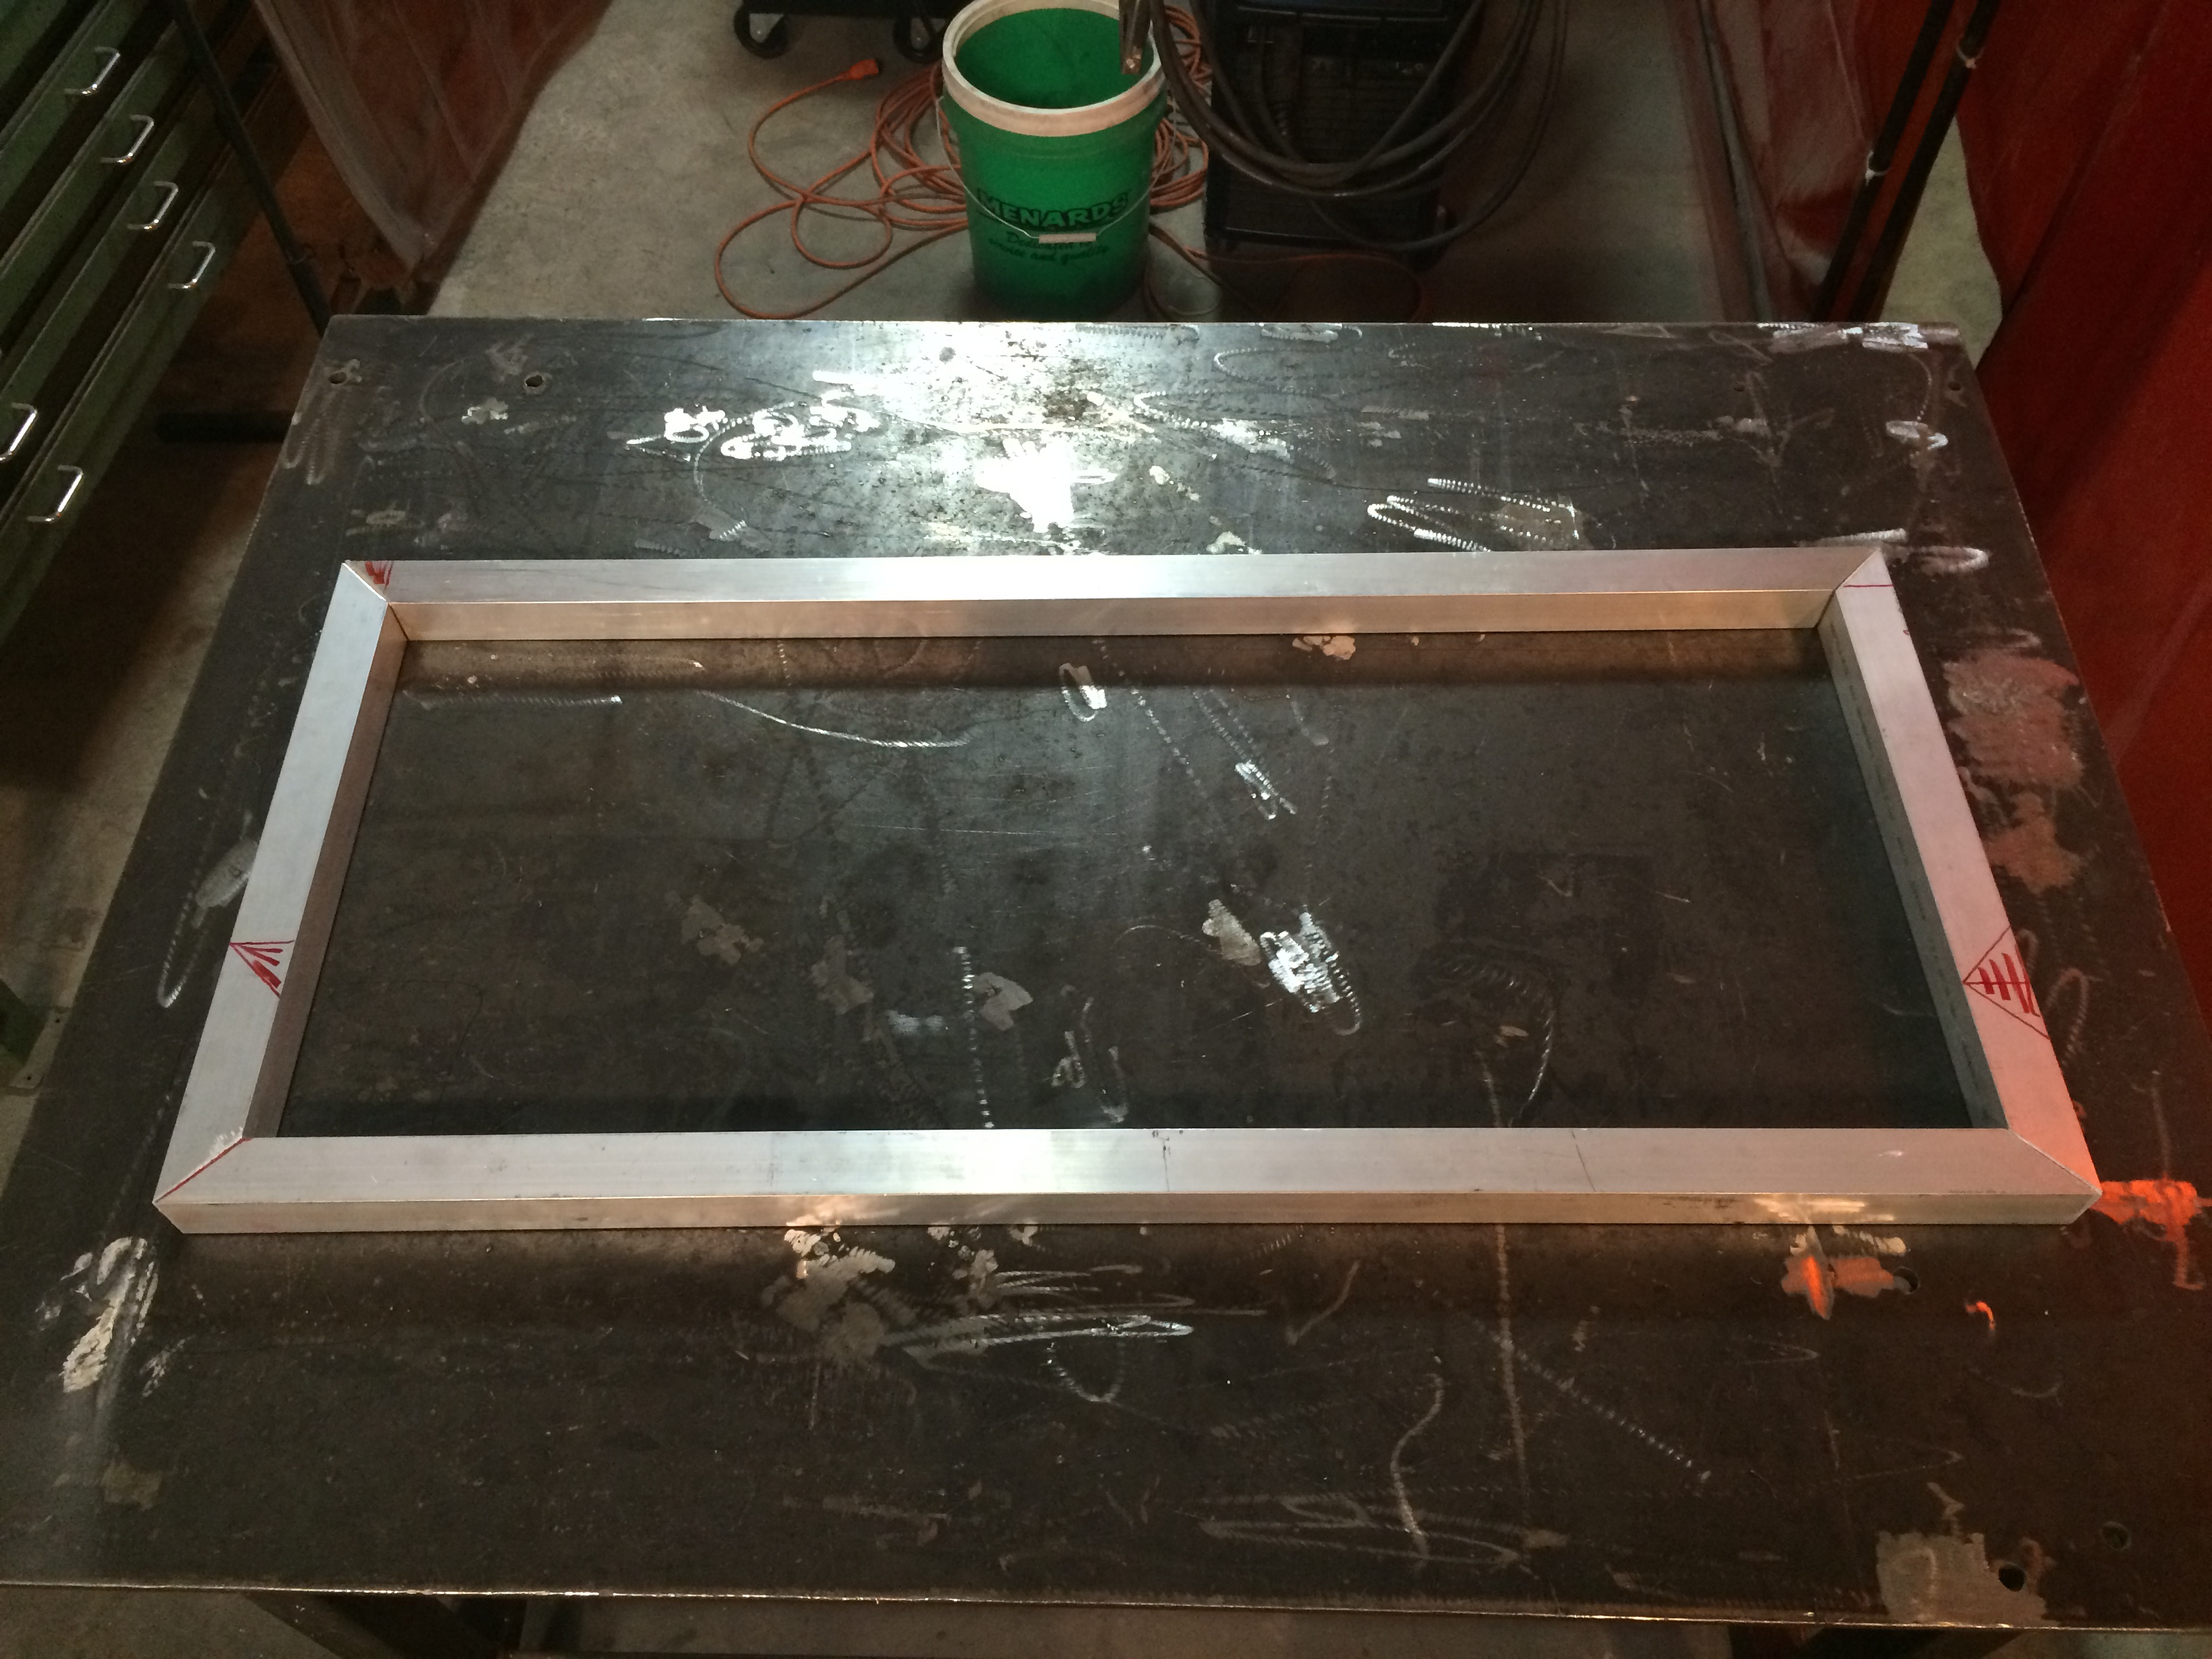
\includegraphics[width=0.6\textwidth]{resources/img/Frame}
\end{center}
\caption{UGV Frame in Construction \label{systemdiagram}}
\end{figure}

\end{enumerate}



%%%%%%%%%%%%%%%%%%%%%%%%%%%%%%%%%%%%%%%%%%%%%%%%%%%%%%%%%%%%%%%%%%%%%%%%%%%%%%%%%%%%
\section{Sprint Report \#6}
Weeks March 23, 2015 to April 10, 2015:
The focus of the final sprint is to integrate all of the components of the project.

\begin{enumerate}

\item UGV

During Sprint 6, the worm gear used for controlling the steering system via a motor was installed using a bracket which secured the motor drive in place. Wiring the motor controls was done by Samuel Carroll, and Hafiza Farzami worked on the motor controls for the drive system. On the way to the design fair, the bracket securing the motor for the drive system was shifted out of alignment. A new, more rigid bracket will need to be installed in order to facilitate steering for the ground vehicle in the future.

\item UAV 

Autonomy has been acheived with the aerial vehicle. The vehicle is capable of Auto-takeoff when set to autonomous mode by a remotely connected computer.

\item Control Panel

The control panel has been integrated into the software architecture and handles the display of the UAV data. The camera feed from the UAV is displayed, as well as the relevant tracking information sent from cv\_tracker and ar\_track\_alvar.

\item Craft Orientation

The cv\_tracker package has been re-structured to read the same raw video feed that ar\_track\_alvar subscribes to, instead of initializing its own camera feed. This cuts down processor load by sharing an already existing camera feed instead of running two separate feeds simultaneously.

\item Navigation

The wavefront algorithm for the path planning for the ground vehicle has been completed. the design details are located in Section~\ref{softwarepathplanning} of the design document.

\end{enumerate}